\documentclass[12pt]{article}

\usepackage{graphicx}
\usepackage{hyperref}
\usepackage{listings}

\setlength{\textheight}{8.5in}
\setlength{\headheight}{.25in}
\setlength{\headsep}{.25in}
\setlength{\topmargin}{0in}
\setlength{\textwidth}{6.5in}
\setlength{\oddsidemargin}{0in}
\setlength{\evensidemargin}{0in}

\title{PartyUp Internals}
\author{David Gilhooley, Lance Goodridge, Blake Lawson, and Graham Turk}

\begin{document}

\pagestyle{plain}

\maketitle

%%---------------------------------------------------------------------------------------------------
%% Introduction
%%---------------------------------------------------------------------------------------------------

\section{Overview}

PartyUp is an iOS app written in Swift.
The app's back end is hosted on an Amazon Web Services (AWS)
EC2 instance running Ubuntu.
The back end is built using the Django web framework and uses
a MySQL database.
PartyUp uses Git for version control and the code for the project is 
hosted on \href{https://github.com/}{GitHub}.
The iOS code and back end code can be found at 
\url{https://github.com/BDGL-Hacks/iOS-333} and
\url{https://github.com/BDGL-Hacks/backend-333} respectively.

The front end iOS app interacts with the back end API through HTTP requests.
The iOS client sends a POST request that indicates which API function to call 
to the Django application on the AWS instance, and the server returns a JSON object that 
includes the information requested by the client.
All of the functions in the PartyUp API are documented on GitHub
in the \href{https://github.com/BDGL-Hacks/backend-333/wiki}{project wiki},

%%---------------------------------------------------------------------------------------------------
%% Front End
%%---------------------------------------------------------------------------------------------------

\section{Implementation: Front End}

The project's iOS code is written in the Swift programming language in the Xcode development environment.
You can build and run the project using one of the simulators in Xcode or
by plugging in a registered Apple device.
The code design follows the traditional Model-View-Controller (MVC) paradigm.
On the UI side, we used Xcode's interface builder tool to
create the views the user interacts with.
The interface builder generates XML code in the \texttt{Main.storyboard file},
which can be inspected in any text editor.

Each view is linked with a view controller class
which dictates how to render the view and handle the user's actions. 
The view controllers interact with model classes to fetch information 
that is displayed on the screen. 
The view controllers also stores information the user inputs. 
The models function as the middlemen between the front end and back end: 
during the creation process the models are areas to store local information 
before the user completes the event or group. When fetching data the models 
test for errors and null values before passing the information to the view controllers.

All model classes call methods of the singleton class \texttt{PartyUpBackend.swift},
which handles information exchange with the back end, including event creation,
push notification queries, and group message retrieval.
Each method in this class prepares a dictionary of post parameters which is
sent via HTTP request to the server through a method called \texttt{sendPostRequest()}.
The \texttt{sendPostRequest()} method converts the returned JSON file from the back end to a dictionary object,
which it then returns to the caller.

We use a class called DataManager.swift to handle key-value lookups of dictionary objects.
All of the data manager's methods are static and require a dictionary (e.g. an event) as an argument.
They return (in proper format) the value associated with whatever key the method name corresponds to. 

Much of the information exchange between view controllers is done in the \texttt{prepareForSegue()} method,
called when the user triggers a segue from one view to another. In prepareForSegue(),
we determine which segue will be executed and then set any variables of the destination view
controller before it displays on screen.
For example, when a user clicks on a table cell in the ``My Events" table,
we pass the cell's associated event dictionary to the event info page's view controller,
where it can render the information accordingly. 

%% LANCE HERE %%

Lance talks about iOS group messaging and push notifications here

%%---------------------------------------------------------------------------------------------------
%% Back End
%%---------------------------------------------------------------------------------------------------

\section{Implementation: Back End}

At a high level, there are a few major components to the back end:
an AWS EC2 instance, an AWS S3 bucket, Pusher, and the Apple Push Notification Service (APNS).
Figure~\ref{fig:stack} contains a graphical representation of the system.

\begin{figure}[h]
    \centering
    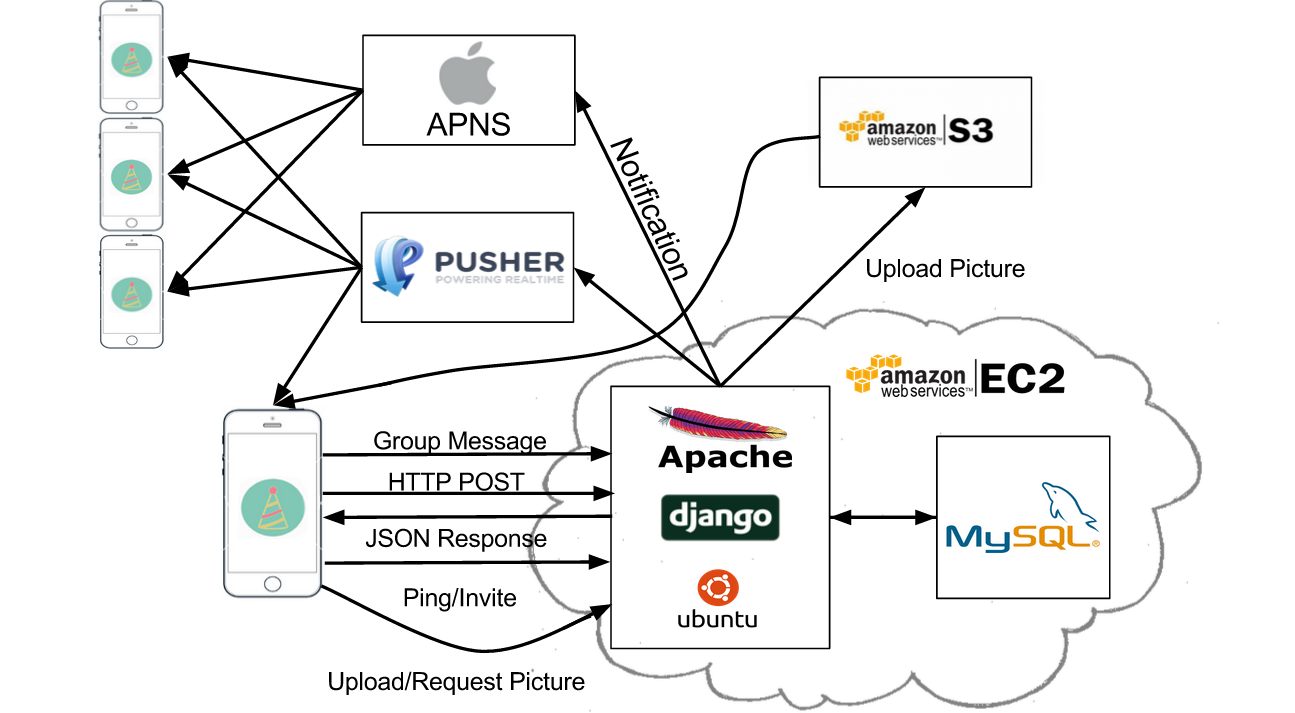
\includegraphics[scale=0.4]{Stack.png}
    \caption{
        A simplified map of the PartyUp back end. 
    }
    \label{fig:stack}
\end{figure}


In this section, we will give an overview each of major components in this system
in the context of the code found in the
\href{https://github.com/BDGL-Hacks/backend-333}{backend-333 directory}.
At the top level, there are a few files and sub-directories.

\texttt{curl.sh} is a short bash script that is basically a wrapper for 
\texttt{cURL} that makes it a little easier to test the back end API.

\texttt{requirements.txt} is a list of Python packages that are needed to
run all of the Python programs within the directory.
All of the packages can be installed using \texttt{pip}, the recommended
Python package manager.
The command
\begin{lstlisting}
    pip install -r requirements.txt
\end{lstlisting}
will install all of the packages at once.

The two directories, \texttt{testdata} and \texttt{partyup} will be covered
in greater detail below.
It should noted that all of the Python files included in these directories
is written to the PEP-8 Python standard.

\subsection{testdata}

This directory contains a Python script, \texttt{filldatabase.py},
which can be used to fill the PartyUp database with test data
found in the accompanying files, \texttt{users.txt} and \texttt{events.txt}.
The files themselves are well documented and contain information about
how to run the script.

\subsection{partyup}

This directory contains the Django project, and thus,
it contains most of the code for the back end.
For the most part, the files are structured in the way you would
expect in your typical Django project
(see \url{https://docs.djangoproject.com/en/1.7/} for an introduction to Django),
although there are a few exceptions.

\end{document}
